\documentclass[11pt]{article}
\usepackage[T1]{fontenc}
\usepackage[utf8]{inputenc}
\usepackage{lmodern,amsmath,amssymb,amsthm,mathtools}
\usepackage{microtype,geometry,booktabs,array,xcolor,hyperref}
\usepackage{tikz}
\usetikzlibrary{arrows.meta,positioning,fit,calc,shapes.geometric}
\geometry{margin=1in}
\hypersetup{colorlinks=true,linkcolor=blue!55!black,citecolor=blue!55!black,urlcolor=blue!55!black}
\newtheorem{theorem}{Theorem}[section]
\newtheorem{proposition}[theorem]{Proposition}
\newtheorem{lemma}[theorem]{Lemma}
\newtheorem{corollary}[theorem]{Corollary}
\newtheorem{remark}[theorem]{Remark}
\newtheorem{definition}[theorem]{Definition}
\newtheorem{example}[theorem]{Example}
\newcommand{\GG}{G}
\newcommand{\HH}{\overline G}
\newcommand{\OO}[1]{O_{#1}}
\newcommand{\VV}{V(G)}
\newcommand{\NP}[1]{N_G[#1]}
\newcommand{\CC}[1]{C(#1)}
\newcommand{\FF}[1]{F(#1)}
\newcommand{\DD}[2]{D_{#1}(#2)}
\title{Blind Discovery of Octahedral Retractions\\
\large Structural Obstructions, Conflict-Guided Repair, and the Fourth Clique Iterate of the Snub Disphenoid}
\author{Research note accompanying the \texttt{pycliques} algorithms}
\date{21 November 2026}
\begin{document}
\maketitle
\begin{abstract}
We develop general, graph-independent techniques for constructing a retraction
onto an induced octahedral graph \(O_d=\overline{dK_2}\). The main tools are
incremental antipodal-pair selection, partial retraction fibers,
an exact forced-subgraph obstruction, binary-domain 2-SAT, conflict learning,
minimum hitting sets for nonlocal pair replacement, and an exact bounded
completion algorithm directed by complement domination. These techniques
were developed to rediscover a retraction \(K^4(S)\to O_{24}\), where \(S\)
is the eight-vertex snub disphenoid graph. We explain the logically exact
certificates, their relation to earlier special-retraction theorems,
and the distinction between heuristic discovery and proof by independent
verification. The code contains no saved snub-specific antipodal pairs.
\end{abstract}
\tableofcontents

\section{Conventions and the target problem}
All graphs are finite, undirected, simple, and loopless. A \emph{complete}
is a nonempty set of pairwise adjacent vertices; a \emph{clique} is an
inclusion-maximal complete. We identify a graph with its vertex set when
no ambiguity arises. A graph morphism \(f:G\to H\) may send adjacent
vertices to \emph{adjacent or equal} vertices. A \emph{retraction}
\(r:G\to T\) fixes every vertex of an induced subgraph \(T\subseteq G\).
The clique graph \(K(G)\) is the intersection graph of the maximal cliques
of \(G\). Iteration is denoted by \(K^j(G)\).

Write
\[
   O_d=\overline{dK_2},\qquad
   V(O_d)=\{a_1,b_1,\ldots,a_d,b_d\},
\]
where the only missing edges between distinct vertices are
\(a_ib_i\), for \(1\le i\le d\). Each pair \(p_i=\{a_i,b_i\}\)
is called an \emph{antipodal pair}, and \(\bar a_i=b_i\),
\(\bar b_i=a_i\). Any different antipodal pairs are completely joined.
An induced \(O_d\) can therefore be encoded by its \(d\) pairwise compatible
nonedges.

\begin{figure}[ht]
\centering
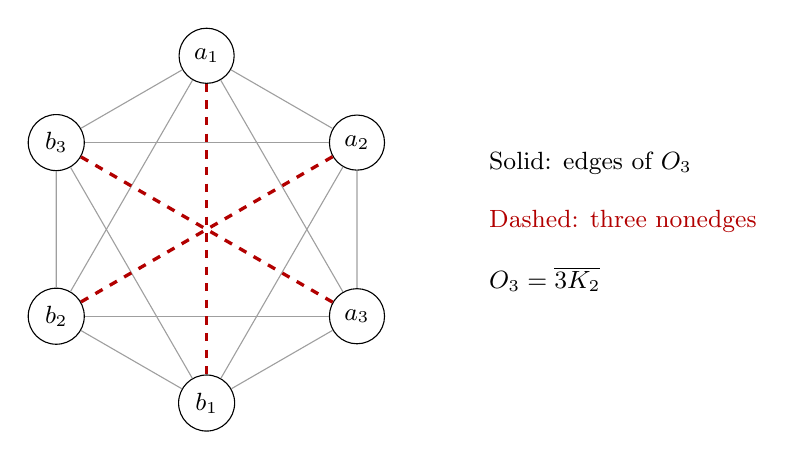
\begin{tikzpicture}[scale=1.05, every node/.style={font=\small}]
  \foreach \name/\angle in {a_1/90,a_2/30,a_3/-30,b_1/-90,b_2/-150,b_3/150}{
    \node[circle,draw=black,fill=white,minimum size=7mm] (\name) at (\angle:2.1) {$\name$};
  }
  \foreach \x/\y in {a_1/a_2,a_1/a_3,a_1/b_2,a_1/b_3,
    a_2/a_3,a_2/b_1,a_2/b_3,a_3/b_1,a_3/b_2,
    b_1/b_2,b_1/b_3,b_2/b_3}{
    \draw[gray!75,thin] (\x)--(\y);
  }
  \foreach \x/\y in {a_1/b_1,a_2/b_2,a_3/b_3}{
    \draw[red!70!black,dashed,very thick] (\x)--(\y);
  }
  \node[align=left,anchor=west] at (3.3,.8) {Solid: edges of $O_3$};
  \node[align=left,anchor=west,text=red!70!black] at (3.3,.1) {Dashed: three nonedges};
  \node[align=left,anchor=west] at (3.3,-.6) {$O_3=\overline{3K_2}$};
\end{tikzpicture}
\caption{The octahedral graph \(O_3\). Dashed segments represent the antipodal nonedges, not edges of the graph.}
\label{fig:octahedron}
\end{figure}

A fundamental classical fact is
\(K(O_d)\cong O_{2^{d-1}}\), for \(d\ge2\), and hence
\(O_d\) is clique divergent when \(d\ge3\) \cite{LarPizVil2019,NeuLara1978}.
Neumann-Lara's retraction theorem states that if \(T\) is a
clique-divergent retract of \(G\), then \(G\) is clique divergent
\cite{LarPizVil2008,LarPizVil2019}. It is therefore enough to
construct a retraction onto an induced \(O_d\), \(d\ge3\).

\section{Compatible nonedges and complement domination}
For a set \(P\) of antipodal pairs inducing \(O_k\) in \(G\), put
\[
\CC P=\bigcap_{a\in\bigcup P}N_G[a].
\]
If \(P\) is empty, let \(\CC P=\VV\). Every antipodal pair that can
be added to \(P\) has both endpoints in \(\CC P\). Conversely,
a nonedge \(uv\) with \(u,v\in\CC P\) is compatible with every pair
in \(P\), and the new common neighborhood is
\(\CC{(P\cup\{\{u,v\}\})}=\CC P\cap N_G[u]\cap N_G[v]\).

\begin{lemma}[Necessary domination]\label{lem:domination}
If \(G\) retracts onto an induced \(T\cong O_d\), then
\(\bigcap_{a\in V(T)}N_G[a]=\varnothing\).
\end{lemma}
\begin{proof}
Suppose \(x\) belongs to the intersection and let \(r(x)=a\in T\).
The antipode \(\bar a\) belongs to \(T\), so \(r(\bar a)=\bar a\).
But \(x\) is adjacent to \(\bar a\) and \(a\) is not adjacent to
\(\bar a\), contradicting the morphism condition. The case \(x=a\)
is impossible as well, because \(a\notin N_G[\bar a]\).
\end{proof}

\begin{remark}
The empty intersection is necessary, not sufficient. Every
complement-dominating induced octahedron must still pass a separate
retraction test; this distinction was decisive in the snub search.
\end{remark}

\section{Constructing a retraction through its fibers}
We first give an exact constructive criterion.
\begin{theorem}[Antipodal fiber criterion]\label{thm:fibers}
Let \(T\cong O_d\) be induced in \(G\), with antipodal pairs
\(\{a_i,b_i\}\). The following are equivalent:
\begin{enumerate}
\item There is a retraction \(r:G\to T\).
\item The vertex set of \(G\) admits a partition
\(V(G)=\bigsqcup_{i=1}^d(A_i\sqcup B_i)\) such that
\(a_i\in A_i\), \(b_i\in B_i\), and \(A_i\) is anticomplete to \(B_i\)
for every \(i\).
\end{enumerate}
\end{theorem}
\begin{proof}
If \(r\) is a retraction, put \(A_i=r^{-1}(a_i)\) and
\(B_i=r^{-1}(b_i)\). These fibers partition \(V(G)\) and contain
the anchors. If \(x\in A_i\), \(y\in B_i\) were adjacent, their
images would be the nonadjacent vertices \(a_i,b_i\), a contradiction.

Conversely, let such a partition be given, and define \(r(x)=a_i\)
for \(x\in A_i\), \(r(x)=b_i\) for \(x\in B_i\).
It fixes all vertices of \(T\). If \(xy\in E(G)\), the images
cannot be opposite endpoints of the same antipodal pair, because
\(A_i\) and \(B_i\) are anticomplete. All remaining pairs of
images are adjacent or equal in \(T\). Thus \(r\) is a retraction.
\end{proof}

The criterion also applies to \emph{partial} maps on a subset
\(X\subseteq V(G)\): if we select a partial induced \(O_k\) and
pairwise disjoint fibers \(A_i,B_i\subseteq X\) that satisfy the
same constraints, we have a valid homomorphism \(G[X]\to O_k\).
This provides a simultaneous embedding-and-map search; each step
adds an antipodal nonedge and a complete bipartite subgraph between
its fibers in the complement \(\overline G\).

\begin{figure}[ht]
\centering
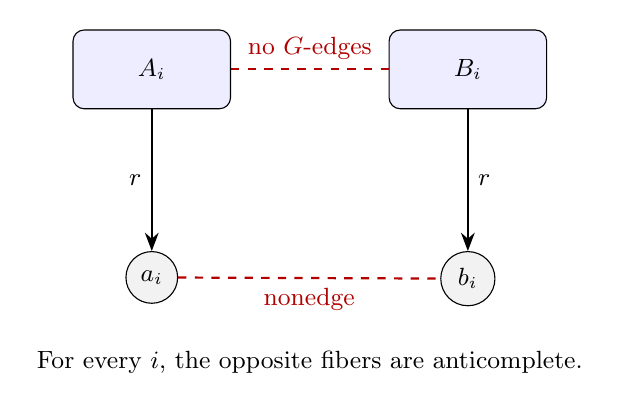
\begin{tikzpicture}[>=Stealth, node distance=10mm and 13mm, every node/.style={font=\small}]
  \node[draw,rounded corners,fill=blue!7,minimum width=20mm,minimum height=10mm] (A) {$A_i$};
  \node[draw,rounded corners,fill=blue!7,right=20mm of A,minimum width=20mm,minimum height=10mm] (B) {$B_i$};
  \node[below=18mm of A,circle,draw,fill=gray!10] (a) {$a_i$};
  \node[below=18mm of B,circle,draw,fill=gray!10] (b) {$b_i$};
  \draw[->,thick] (A)--node[left] {$r$}(a);
  \draw[->,thick] (B)--node[right] {$r$}(b);
  \draw[red!70!black,dashed,thick] (A)--node[above] {no $G$-edges}(B);
  \draw[red!70!black,dashed,thick] (a)--node[below] {nonedge}(b);
  \node[below=8mm of $(a)!.5!(b)$] {For every $i$, the opposite fibers are anticomplete.};
\end{tikzpicture}
\caption{Fibers of a retraction onto one antipodal pair. Edges between other fibers are unrestricted.}
\label{fig:fibers}
\end{figure}

\section{The forced-subgraph obstruction}
A partial octahedron constrains many vertices even before the remaining
antipodal pairs are known. Define
\[
\FF P=\bigcup P\;\cup\;
\bigl\{x\in V(G):N_{\overline G}(x)\cap\CC P=\varnothing\bigr\},
\]
where \(N_{\overline G}(x)\) is the \emph{open} neighborhood in the
complement. Thus every vertex of \(\FF P\setminus\bigcup P\) is
adjacent to every possible future anchor in \(\CC P\).

\begin{theorem}[Essential forced-subgraph obstruction]
\label{thm:forced}
Let \(P\) induce \(O_k\) in \(G\), and suppose an extension
\(T\cong O_d\), containing all pairs of \(P\), is the target of a
retraction \(r:G\to T\). Then
\[
       r(\FF P)\subseteq\bigcup P,
       \qquad r|_{G[\FF P]}:G[\FF P]\longrightarrow G[\bigcup P]
\]
is a retraction.
\end{theorem}
\begin{proof}
Every new anchor \(t\in T\setminus\bigcup P\) lies in \(\CC P\),
as does its antipode \(\bar t\). If \(x\in\FF P\setminus\bigcup P\),
then \(x\) is adjacent to \(\bar t\). If \(r(x)=t\), the edge
\(x\bar t\) would be mapped to the nonedge \(t\bar t\), a
contradiction. Hence \(r(x)\) is not a new anchor. All old
anchors are fixed by \(r\), so the restriction has image in
\(\bigcup P\), fixes those vertices, and preserves edges.
\end{proof}

\begin{corollary}[Monotonicity of partial conflicts]
\label{cor:monotone}
If \(G[\FF P]\) does not retract onto \(G[\bigcup P]\), no induced
octahedron extending \(P\) can be a retract of \(G\).
Moreover, if \(Q\supseteq P\) consists of pairwise compatible
antipodal pairs, the obstruction persists: no retracting extension
of \(Q\) exists either.
\end{corollary}
\begin{proof}
The first statement is the contrapositive of
Theorem~\ref{thm:forced}. Every retracting extension of \(Q\)
would also be an extension of \(P\); hence the second follows.
\end{proof}

For a vertex \(x\in\FF P\), define its allowed old-anchor images by
\[
\DD P x=\begin{cases}
\{x\},&x\in\bigcup P,\\
\{\bar a:a\in\bigcup P,\ xa\notin E(G)\},&x\notin\bigcup P.
\end{cases}
\]
Indeed, the only image of \(x\) forbidden by an edge \(xa\) to a
fixed anchor \(a\) is \(\bar a\). In particular,
\(\DD P x=\varnothing\) certifies an impossible extension.

\begin{theorem}[Sound binary-domain 2-SAT obstruction]
\label{thm:twosat}
Consider the vertices \(x\in\FF P\) with
\(|\DD P x|\le2\). For each domain of size two, introduce one Boolean
variable selecting one of its two images. For each edge \(xy\) between
such vertices and each forbidden choice
\((s,t)\in\DD P x\times\DD P y\) with \(t=\bar s\), add the clause
\(\neg(x\mapsto s)\lor\neg(y\mapsto t)\).
If the resulting 2-SAT instance is unsatisfiable, no octahedral
extension of \(P\) is a retract of \(G\).
\end{theorem}
\begin{proof}
Every retracting extension induces a retraction
\(G[\FF P]\to O_k\) by Theorem~\ref{thm:forced}; its vertex images
belong to \(\DD P x\). The restriction to the selected vertices
therefore assigns each Boolean variable and satisfies every clause,
since an edge may not map to opposite anchors. Unsatisfiability
contradicts this necessary assignment.
\end{proof}

\begin{example}[A binary-domain contradiction]
Let \(P=O_3\) with pairs \((0,1),(2,3),(4,5)\). Add three vertices
\(x,y,z\) joined by the edges \(xy,yz\), and arrange their edges to
the anchors so that
\[
    \DD P x=\{2\},\qquad \DD P y=\{1,3\},
    \qquad \DD P z=\{0\}.
\]
The edge \(xy\) forces \(y\mapsto1\) (since \(2\) and \(3\)
are nonadjacent), whereas \(yz\) forces \(y\mapsto3\)
(since \(0\) and \(1\) are nonadjacent). This is impossible,
although no edge directly joins two vertices with singleton domains
forced to opposite anchors.
\end{example}

The 2-SAT obstruction is sufficient for rejection but not for acceptance.
Vertices with three or more candidate old-anchor images are not
constrained by the binary-domain test; even a satisfiable instance
need not extend to a retraction.

\section{Conflict cores and optimal nonlocal repair}
A set \(Q\subseteq P\) of antipodal pairs is a \emph{conflict}
if the forced-subgraph 2-SAT screen certifies failure on \(Q\).
It is \emph{deletion-minimal} if the screen no longer certifies
failure after deleting any one pair. An algorithm may remove
pairs one by one as long as the screen remains negative; the result
is a logically sound conflict core. An iteration limit may leave
a valid but non-minimal conflict.

\begin{theorem}[Conflict-hitting theorem]
\label{thm:hitting}
Let \(P=\{p_1,\ldots,p_k\}\) be compatible antipodal pairs and
let \(\mathcal C\) be a family of subsets \(C\subseteq P\), each
proved incompatible with every retracting octahedral extension.
Suppose a modified target retains all pairs of \(P\setminus D\)
and retracts from \(G\). Then
\[
             D\cap C\ne\varnothing
               \qquad\text{for every } C\in\mathcal C.
\]
In particular \(|D|\ge\tau(\mathcal C)\), where \(\tau\) is the
transversal number of this conflict hypergraph.
\end{theorem}
\begin{proof}
If \(D\cap C=\varnothing\), all pairs of \(C\) would remain
in the retracting target. This target would be an extension of
\(C\), contrary to the definition of a conflict.
\end{proof}

\begin{example}[A hitting-set calculation]
Suppose three detected conflicts on five pair indices are
\(C_1=\{1,3\}\), \(C_2=\{2,3\}\), and \(C_3=\{3,5\}\).
Deleting pair 3 intersects all three conflicts, while any
other one-pair deletion misses at least one. Hence
\(\tau(\mathcal C)=1\) and \(D=\{3\}\) is the unique optimal
one-pair repair. This does \emph{not} guarantee a retracting completion.
\end{example}

\begin{figure}[ht]
\centering
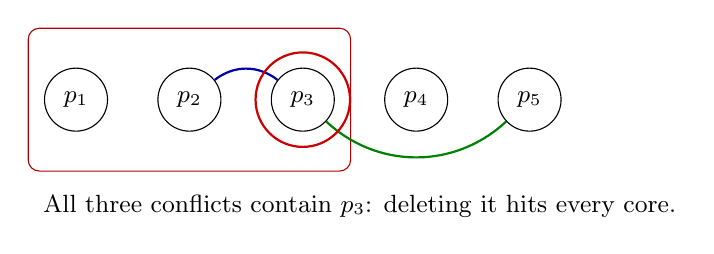
\begin{tikzpicture}[every node/.style={font=\small},scale=.9]
  \foreach \i in {1,...,5}{
    \node[draw,circle,minimum size=8mm,fill=white] (p\i) at (1.6*\i,0) {$p_{\i}$};
  }
  \node[draw=red!70!black,rounded corners,fit=(p1)(p3),inner xsep=2mm,inner ysep=5mm] (c1) {};
  \draw[blue!65!black,thick] (p2) to[bend left=38] (p3);
  \draw[green!50!black,thick] (p3) to[bend right=43] (p5);
  \node[draw,circle,thick,red!80!black,minimum size=12mm] at (p3) {};
  \node[anchor=west] at (1,-1.5) {All three conflicts contain $p_3$: deleting it hits every core.};
\end{tikzpicture}
\caption{Schematic conflict hypergraph. The red ring highlights the unique one-pair hitting set for the illustrated family.}
\end{figure}

Positive integer weights \(w_i\) may be assigned to pairs to discourage
removal of large or computationally useful fibers. The resulting exact
finite optimization problem is
\[
 \min \sum_{i\in D}w_i
 \quad\text{subject to}\quad D\cap C\ne\varnothing
 \text{ for every }C\in\mathcal C.
\]
The implementation uses branch-and-bound on a smallest uncovered
conflict, with no assumption that a hitting set ensures success.

\section{Exact domination-directed octahedral completion}
Let \(P\) be fixed and let \(r=d-|P|\) pairs still be required.
An extension must choose \(r\) mutually compatible nonedges inside
\(G[\CC P]\), making the final common closed neighborhood empty.
The next theorem yields an exhaustive branching rule.

\begin{theorem}[Constrained-neighbor branching]
\label{thm:pivot}
Let \(P\) induce an \(O_k\) in \(G\), and let \(C=\CC P\ne\varnothing\).
For any \(w\in C\), every complement-dominating extension of \(P\)
contains a new antipodal pair \(\{u,v\}\subseteq C\) with
\(u\in N_{\overline G}(w)\cap C\) or
\(v\in N_{\overline G}(w)\cap C\).
Thus one may branch only on new compatible nonedges having an endpoint
in \(N_{\overline G}(w)\cap C\). If this set is empty, no such
extension exists.
\end{theorem}
\begin{proof}
Since the final common closed neighborhood is empty, some
new endpoint \(u\) must fail to be a closed neighbor of \(w\).
Because \(w\in C\), every old endpoint is a closed neighbor of \(w\);
thus \(u\) belongs to a new antipodal pair and is distinct and
nonadjacent to \(w\). This is precisely
\(u\in N_{\overline G}(w)\cap C\). The pairs of an induced
\(O_d\) are mutually compatible, so their order can be changed to
put this pair first. Hence the branching is exhaustive.
\end{proof}

\begin{corollary}[Correctness of bounded completion]\label{cor:complete}
The recursion that chooses a pivot \(w\), branches on every eligible
antipodal pair containing a nonneighbor of \(w\), and updates
\(C\gets C\cap N_G[u]\cap N_G[v]\), is complete provided it
explores all branches. It returns a valid complement-dominating
\(O_d\) if successful. If all branches fail, nonexistence of such
an extension is proved. If a state budget is reached, the outcome
is inconclusive.
\end{corollary}
\begin{proof}
Every possible completion is represented in the first step by
Theorem~\ref{thm:pivot}; apply the same reasoning inductively to
the remaining pairs. At zero remaining pairs, domination holds
exactly if \(C=\varnothing\). Pruning when \(|C|<2r\) or when
there are fewer than \(r\) nonedges in \(G[C]\) is necessary,
so it cannot remove a valid completion. Recording only fully
exhausted states is sound; a truncated state cannot justify
exhaustion.
\end{proof}

A practical pivot is the vertex \(w\in C\) with the fewest
nonneighbors in \(G[C]\), which minimizes the initial branching
set. The recursion is still exponential in the worst case; the
bound on explored states is essential for practical use.

\section{Optional auxiliary obstructions}
Two additional necessary conditions can be useful but are not part
of the certified core proof.

\begin{proposition}[Clique-orientation obstruction]
\label{prop:clique-sat}
Let \(T\cong O_d\) be an induced target of a retraction
\(r:G\to T\), and let \(Q\) be any complete of \(G\).
There is a transversal \(B\) selecting one endpoint from every
antipodal pair of \(T\) such that
\(\DD T x\cap B\ne\varnothing\) for every \(x\in Q\).
\end{proposition}
\begin{proof}
The image \(r(Q)\) is complete in \(T\), because an edge may
map to an edge or a vertex. It contains at most one endpoint of
each antipodal pair, and therefore extends to a transversal
\(B\). Since each \(r(x)\in\DD T x\cap B\), the assertion follows.
\end{proof}

The condition is a Boolean CNF satisfiability test on \(d\) choice
variables. Its failure proves that the specified \(T\) is not a
retract; its success is only necessary.

A second option is the integer-programming description of a
dominating induced matching in \(H=\overline G\). Binary variables
\(x_v\in\{0,1\}\) must satisfy
\begin{align*}
\sum_{v\in V(H)}x_v&=2d,\\
\sum_{u\in N_H(v)}x_u&\ge1&& (v\in V(H)),\\
\sum_{u\in N_H(v)}x_u+(\deg_H(v)-1)x_v&\le\deg_H(v)&& (v\in V(H)).
\end{align*}
If \(x_v=1\), the last two inequalities force exactly one selected
neighbor of \(v\), so the selected vertices induce \(dK_2\) in
\(H\); the second inequality ensures domination. Thus the binary
system describes exactly the complement-dominating induced \(O_d\)'s
in \(G\). Infeasibility of its linear relaxation is a sound prune;
LP feasibility is not sufficient. The core reproduction described
below does not require an LP solver.

\section{The snub-disphenoid computation}
Let \(S\) be the eight-vertex snub disphenoid, isomorphic to the graph
with graph6 string \texttt{GQyuzw}. We use the canonical
\(F_{4,4}\) labeling: the two induced paths are
\(0\! -\! 1\! -\! 2\! -\! 3\) and
\(4\! -\! 5\! -\! 6\! -\! 7\), and vertices \(i\in\{0,1,2,3\}\)
and \(4+j\in\{4,5,6,7\}\) are adjacent exactly when
\(i\in\{0,3\}\) or \(j\in\{0,3\}\).

\begin{table}[ht]
\centering
\begin{tabular}{@{}lrr@{}}
\toprule
Graph & Vertices & Edges\\
\midrule
\(S\) & 8 & 18\\
\(K(S)\) & 12 & 46\\
\(K^2(S)\) & 20 & 136\\
\(K^3(S)\) & 56 & 1,196\\
\(K^4(S)\) & 1,076 & 504,360\\
\bottomrule
\end{tabular}
\caption{Clique-graph orders and sizes, recomputed from \(S\) using maximal-clique enumeration.}
\end{table}

The following is an algorithmic discovery trace, not a list of
hardcoded anchors:
\begin{enumerate}
\item A seeded, but coordinate-free, joint-fiber beam search
(seed \texttt{24002}, beam width 12, 25 candidate pairs per step)
finds a partial \(O_{22}\), with a partial morphism defined on
1,014 of the 1,076 vertices.
\item Forced-subgraph screening and repeated deletion minimization
produce 111 sound, deletion-minimal conflict sets among these 22 pairs.
\item Among the \(\binom{22}{7}=170{,}544\) ways to discard seven
of the original pairs, 764 survive the learned conflicts and the
basic residual domination checks.
\item Ranking these repairs by remaining common-neighborhood size
selects one for which exact completion finds nine compatible
new antipodal pairs after 155,244 recursive states, yielding a
complement-dominating induced \(O_{24}\).
\item A separate octahedral retraction CSP finds a complete
projection after 699 search states. Every one of the 1,076 images
and all 504,360 host edges are independently checked.
\end{enumerate}
The result is a verified retraction
\[
       \boxed{K^4(S)\longrightarrow O_{24}.}
\]
Since \(O_{24}\) is clique divergent, the retraction theorem implies
that \(S\) is clique divergent. This provides a new independently
constructed certificate for the known result, not a new proof of the
retraction theorem itself.

\begin{figure}[ht]
\centering
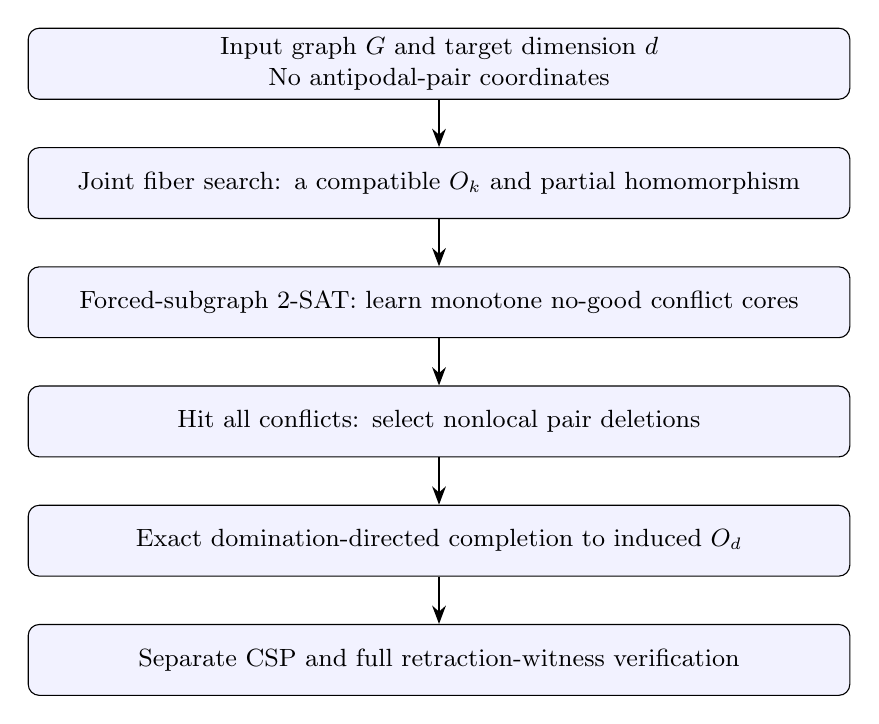
\begin{tikzpicture}[node distance=6mm and 14mm,>=Stealth,
  every node/.style={font=\small},
  box/.style={draw,rounded corners,align=center,text width=10.2cm,
    minimum height=9mm,fill=blue!5}]
\node[box] (s) {Input graph $G$ and target dimension $d$\\No antipodal-pair coordinates};
\node[box,below=of s] (f) {Joint fiber search: a compatible $O_k$ and partial homomorphism};
\node[box,below=of f] (c) {Forced-subgraph 2-SAT: learn monotone no-good conflict cores};
\node[box,below=of c] (h) {Hit all conflicts: select nonlocal pair deletions};
\node[box,below=of h] (e) {Exact domination-directed completion to induced $O_d$};
\node[box,below=of e] (r) {Separate CSP and full retraction-witness verification};
\foreach \x/\y in {s/f,f/c,c/h,h/e,e/r}{\draw[->,thick] (\x)--(\y);}
\end{tikzpicture}
\caption{Generic discovery pipeline. Only the final, independently verified map is a certificate of retraction. Bounded failure at any stage remains inconclusive.}
\label{fig:workflow}
\end{figure}

\section{Relation to special retractions and limitations}
Larri\'on, Piza\~na and Villarroel-Flores proved that, for an induced
\(O_d\subseteq G\), existence of a \emph{special} retraction onto
that target is equivalent to the existence of a transversal clique
of \(O_d\) that is also a clique of \(G\)
\cite[Theorem~3.7]{LarPizVil2019}. Here ``special'' means that for
each antipodal pair one of its endpoints has a singleton fiber.
This yields an elegant direct construction when applicable.

Our method makes no singleton-fiber assumption and uses a general
retraction CSP. A test on the previously certified snub target found
no maximal-clique transversal, so the special-retraction construction
could not have reproduced that particular embedding. This observation
is \emph{target-specific}; it is not a claim that no induced octahedron
in \(K^4(S)\) admits a special retraction.

The discovery algorithm is intentionally heuristic. A different
NetworkX insertion order, random seed, or search budget may produce a
different partial octahedron, and bounded failure cannot rule out a
retract. By contrast, the mathematical obstructions proved in the
preceding sections are sound, and every successful complete projection
can be checked deterministically with no random choices. The supplied
1,076-image JSON certificate uses the graph fingerprint
\begin{center}\small\texttt{0a892f39bb1201d722d19a884b117164b8698a540a6cc1ed6daf99bf802068da}\end{center}
which includes the canonical input vertex ordering and edge set.

\section{Reproducibility in \texttt{pycliques}}
The general software implementation exposes the following APIs:
\begin{quote}\small\ttfamily
screen\_partial\_octahedral\_retraction\\
minimize\_octahedral\_conflict\\
minimum\_octahedral\_repair\\
complete\_dominating\_octahedron\\
discover\_partial\_octahedral\_fibers\\
find\_blind\_octahedral\_retraction
\end{quote}
They accept arbitrary finite simple NetworkX graphs; the first four
have exact mathematical semantics, while the last two include
randomized, bounded discovery. Output labels are the original graph
vertices. The legacy public verifier
\texttt{verify\_retraction\_witness} remains the final authority.

Normal regression tests exercise arbitrary labels, positive examples,
exact negative examples, randomized cross-checks and budgets. The
full snub rediscovery is placed in a separate slow research test.

\begin{thebibliography}{9}
\bibitem{LarPizVil2008}
F. Larri\'on, M. A. Piza\~na, and R. Villarroel-Flores,
\emph{Contractibility and the clique graph operator},
Discrete Mathematics \textbf{308} (2008), 3461--3469.
\url{https://xamanek.izt.uam.mx/map/papers/contractible10w.pdf}.

\bibitem{LarPizVil2019}
F. Larri\'on, M. A. Piza\~na, and R. Villarroel-Flores,
\emph{On the clique behavior of graphs with small constant link},
Ars Combinatoria \textbf{142} (2019), 27--53.
\url{https://xamanek.izt.uam.mx/map/papers/locally6.pdf}.

\bibitem{NeuLara1978}
V. Neumann-Lara,
\emph{On clique-divergent graphs},
in \emph{Probl\`emes combinatoires et th\'eorie des graphes},
Colloques internationaux du CNRS 260, \`Editions du CNRS, Paris, 1978.

\bibitem{Aspvall1979}
B. Aspvall, M. F. Plass, and R. E. Tarjan,
\emph{A linear-time algorithm for testing the truth of certain
quantified Boolean formulas},
Information Processing Letters \textbf{8} (1979), 121--123.
\end{thebibliography}
\end{document}
